\section{Overview: Diversification Rate Estimation} \label{sec:diversification_rate_overview}

Models of speciation and extinction are fundamental to any phylogenetic analysis of macroevolutionary processes (\EG divergence time estimation, diversification rate estimation, continuous and discrete trait evolution, and historical biogeography).
First, a prior model describing the distribution of speciation events over time is critical to estimating phylogenies with branch lengths proportional to time.
Second, stochastic branching models allow for inference of speciation and extinction rates.
These inferences allow us to investigate key questions in evolutionary biology.

Diversification-rate parameters may be included as nuisance parameters of other phylogenetic models---\IE where these diversification-rate parameters are not of direct interest.
For example, many methods for estimating species divergence times---such as \BEAST \citep{Drummond2012}, \MrBayes \citep{Ronquist2012}, and \RevBayes \citep{Hoehna2016b}---implement `relaxed-clock models' that include a constant-rate birth-death branching process as a prior model on the distribution of tree topologies and node ages.
Although the parameters of these `tree priors' are not typically of direct interest, they are nevertheless estimated as part of the joint posterior probability distribution of the relaxed-clock model, and so can be estimated simply by querying the corresponding marginal posterior probability densities.
In fact, this may provide more robust estimates of the diversification-rate parameters, as they accommodate uncertainty in the other phylogenetic-model parameters (including the tree topology, divergence-time estimates, and the other relaxed-clock model parameters).
More recent work, \EG \cite{Heath2014}, uses macroevolutionary models (the fossilized birth-death process) to calibrate phylogenies and thus to infer dated trees.

In these tutorials we focus on the different types of macroevolutionary models to study diversification processes and thus the diversification-rate parameters themselves.
Nevertheless, these macroevolutionary models should be used for other evolutionary questions, when an appropriate prior distribution on the tree and divergence times is needed.


\subsection{Types of Hypotheses for Estimating Diversification Rates}

Many evolutionary phenomena entail differential rates of diversification (speciation -- extinction); \EG adaptive radiation, diversity-dependent diversification, key innovations, and mass extinction.
The specific study questions regarding lineage diversification may be classified within three fundamental categories of inference problems.
Admittedly, this classification scheme is somewhat arbitrary, but it is nevertheless useful, as it allows users to navigate the ever-increasing number of available phylogenetic methods.
Below, we describe each of the fundamental questions regarding diversification rates.

\paragraph{(1) Diversification-rate through time estimation}\textit{What is the (constant) rate of diversification in my study group?} 
The most basic models estimate parameters of the stochastic-branching process (\IE rates of speciation and extinction, or composite parameters such as net-diversification and relative-extinction rates) under the assumption that rates have remained constant across lineages and through time; \IE under a constant-rate birth-death stochastic-branching process model \citep{Nee1994b}.
Extensions to the (basic) constant-rate models include diversification-rate variation through time \citep{Stadler2011,Hoehna2015a}.
First, we might ask whether there is evidence of an episodic, tree-wide increase in diversification rates (associated with a sudden increase in speciation rate and/or decrease in extinction rate), as might occur during an episode of adaptive radiation.
A second question asks whether there is evidence of a continuous/gradual decrease in diversification rates through time (associated with decreasing speciation rates and/or increasing extinction rates), as might occur because of diversity-dependent diversification (\IE where competitive ecological interactions among the species of a growing tree decrease the opportunities for speciation and/or increase the probability of extinction, \EG \cite{Hoehna2014a}).
Third, we can ask whether changes in diversification rates are correlated with environmental factors, such as environmental CO\textsubscript{2} or temperature \citep{Condamine2013}.
A final question in this category asks whether our study tree was impacted by a mass-extinction event (where a large fraction of the standing species diversity is suddenly lost, \EG \cite{May2016}).
The common theme of these studies is that the diversification process is tree-wide, that is, all lineages of the study group have the exact same rates at a given time.



\paragraph{(2) Diversification-rate variation across branches estimation}\textit{Is there evidence that diversification rates have varied significantly across the branches of my study group?}
Models have been developed to detect departures from rate constancy across lineages; these tests are analogous to methods that test for departures from a molecular clock---\IE to assess whether substitution rates vary significantly across lineages \citep{Alfaro2009,Rabosky2014a}.
These models are important for assessing whether a given tree violates the assumptions of rate homogeneity among lineages.
Furthermore, these models are important to answer questions such as:
\textit{What are the branch-specific diversification rates?}; and
\textit{Have there been significant diversification-rate shifts along branches in my study group, and if so, how many shifts, what magnitude of rate-shifts and along which branches?}


\paragraph{(3) Character-dependent diversification-rate estimation}\textit{Are diversification rates correlated with some variable in my study group?}
Character-dependent diversification-rate models aim to identify overall correlations between diversification rates and organismal features (binary and multi-state discrete morphological traits, continuous morphological traits, geographic range, etc.).
For example, one can hypothesize that a binary character, say if an organism is herbivorous/carnivorous or self-compatible/self-incompatible, impact the diversification rates.
Then, if the organism is in state 0 (\EG is herbivorous) it has a lower (or higher) diversification rate than if the organism is in state 1 (\EG carnivorous) \citep{Maddison2007}.


\section{Diversification Rate Models} \label{sec:models}

We begin this section with a general introduction to the stochastic birth-death branching process that underlies inference of diversification rates in \RevBayes.
This primer will provide some details on the relevant theory of stochastic-branching process models.
We appreciate that some readers may want to skip this somewhat technical primer; however, we believe that a better understanding of the relevant theory provides a foundation for performing better inferences.
We then discuss a variety of specific birth-death models, but emphasize that these examples represent only a tiny fraction of the possible diversification-rate models that can be specified in \RevBayes.

\subsection{The birth-death branching process}
Our approach is based on the \textit{reconstructed evolutionary process} described by \cite{Nee1994b}; a birth-death process in which only sampled, extant lineages are observed.
Let $N(t)$ denote the number of species at time $t$.
Assume the process starts at time $t_1$ (the `crown' age of the most recent common ancestor of the study group, $t_\text{MRCA}$) when there are two species.
Thus, the process is initiated with two species, $N(t_1) = 2$.
We condition the process on sampling at least one descendant from each of these initial two lineages; otherwise $t_1$ would not correspond to the $t_\text{MRCA}$ of our study group.
Each lineage evolves independently of all other lineages, giving rise to exactly one new lineage with rate $b(t)$ and losing one existing lineage with rate $d(t)$ (Figure~\ref{fig:BirthDeathShift} and Figure~\ref{fig:BDP}).
Note that although each lineage evolves independently, all lineages share both a common (tree-wide) speciation rate $b(t)$ and a common extinction rate $d(t)$ \citep{Nee1994b,Hoehna2015a}.
Additionally, at certain times, $t_{\mathbb{M}}$, a mass-extinction event occurs and each species existing at that time has the same probability, $\rho$, of survival.
Finally, all extinct lineages are pruned and only the reconstructed tree remains (Figure \ref{fig:BirthDeathShift}).

\begin{figure}[h]
\centering
       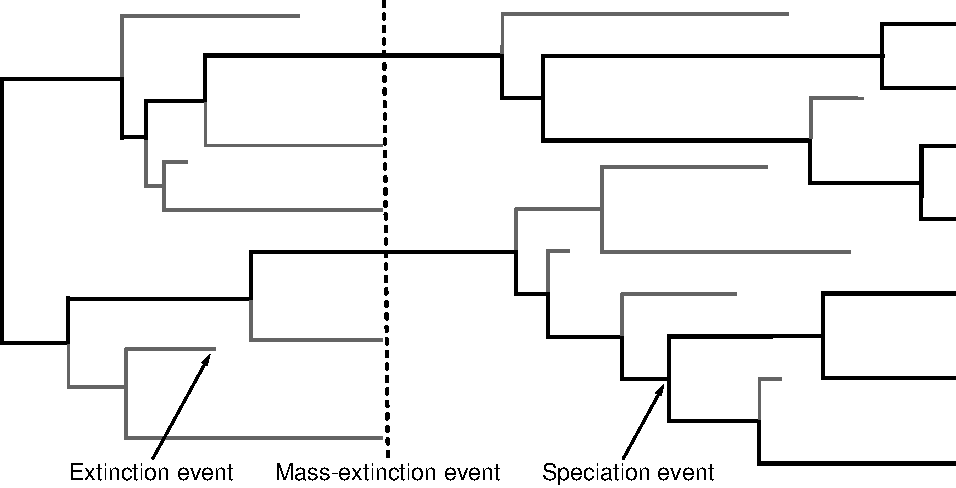
\includegraphics[width=0.8\textwidth]{\ResourcePath figures/BirthDeathShift.pdf}
   \caption{A realization of the  birth-death process with mass extinction.
   Lineages that have no extant or sampled descendant are shown in gray and surviving lineages are shown in a thicker black line.}
\label{fig:BirthDeathShift}
\end{figure}

\begin{figure}[!htbp]
  	\begin{center}
  		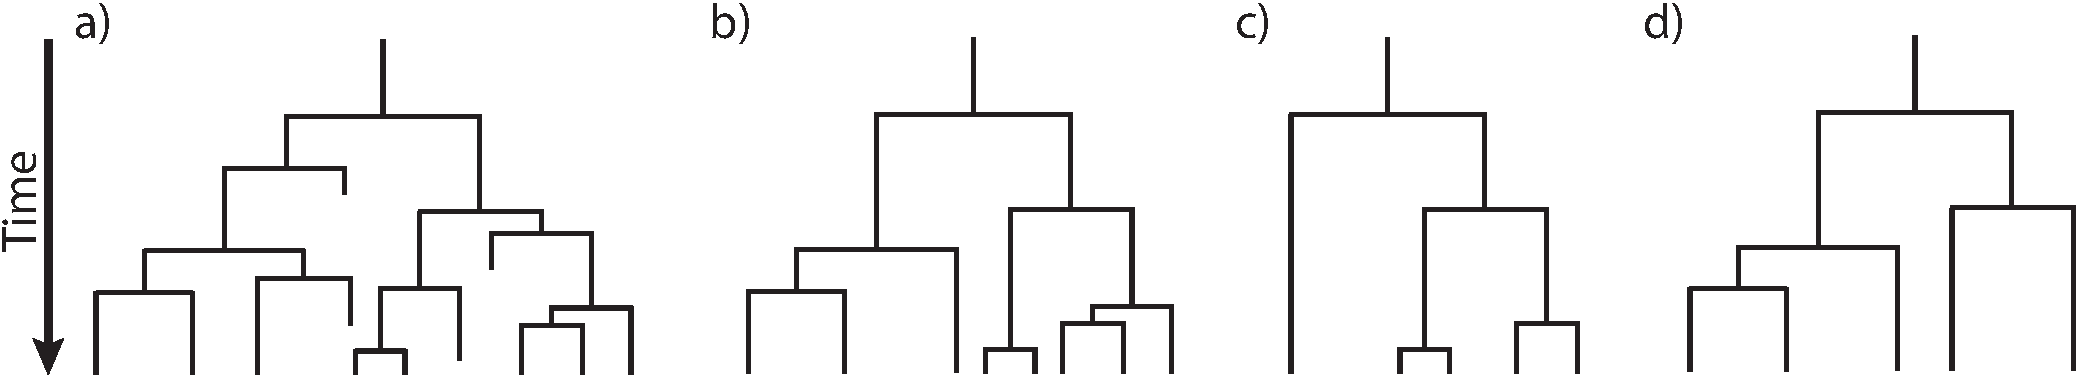
\includegraphics[width=\textwidth]{\ResourcePath figures/birth-death-sketch.pdf}
		\caption{
		{\bf Examples of trees produced under a birth-death process.}
		The process is initiated at the first speciation event (the `crown-age' of the MRCA) when there are two initial lineages.
		At each speciation event the ancestral lineage is replaced by two descendant lineages.
		At an extinction event one lineage simply terminates.
		(A) A complete tree including extinct lineages.
		(B) The reconstructed tree of tree from A with extinct lineages pruned away.
		(C) A \emph{uniform} subsample of the tree from B, where each species was sampled with equal probability, $\rho$.
		(D) A \emph{diversified} subsample of the tree from B, where the species were selected so as to maximize diversity.}
	\label{fig:BDP}
  	\end{center}
\end{figure}

To condition the probability of observing the branching times on the survival of both lineages that descend from the root, we divide by $P(N(T) > 0 | N(0) = 1)^2$.
Then, the probability density of the branching times, $\mathbb{T}$, becomes
\begin{align*}
P(\mathbb{T}) = \frac{\overbrace{P(N(T) = 1 \mid N(0) = 1)^2}^{\text{both initial lineages have one descendant}}}{ \underbrace{P(N(T) > 0 \mid N(0) = 1)^2}_{\text{both initial lineages survive}} } \times \prod_{i=2}^{n-1} \overbrace{i \times b(t_i)}^{\text{speciation rate}} \times \overbrace{P(N(T) = 1 \mid N(t_i) = 1)}^\text{lineage has one descendant},
\end{align*}
and the probability density of the reconstructed tree (topology and branching times) is then
\begin{align}
P(\Psi) = \; & \frac{2^{n-1}}{n!(n-1)!} \times \left( \frac{P(N(T) = 1 \mid N(0) = 1)}{P(N(T) > 0 \mid N(0) = 1)} \right)^2 \nonumber\\
		  \; & \times \prod_{i=2}^{n-1} i \times b(t_i) \times P(N(T) = 1 \mid N(t_i) = 1)
	\label{eq:tree_probability}
\end{align}

We can expand Equation~(\ref{eq:tree_probability}) by substituting $P(N(T) > 0 \mid N(t) =1)^2 \exp(r(t,T))$ for $P(N(T) = 1 \mid N(t) = 1)$, where $r(u,v) = \int^v_u d(t)-b(t)dt$; the above equation becomes
\begin{align}
P(\Psi) = \; & \frac{2^{n-1}}{n!(n-1)!} \times \left( \frac{P(N(T) > 0 \mid N(0) =1 )^2 \exp(r(0,T))}{P(N(T) > 0 \mid N(0) = 1)} \right)^2 \nonumber\\
		  \; & \times \prod_{i=2}^{n-1} i \times b(t_i) \times P(N(T) > 0 \mid N(t_i) = 1)^2 \exp(r(t_i,T)) \nonumber\\
		= \; & \frac{2^{n-1}}{n!} \times \Big(P(N(T) > 0 \mid N(0) =1 ) \exp(r(0,T))\Big)^2 \nonumber\\
		  \; & \times \prod_{i=2}^{n-1} b(t_i) \times P(N(T) > 0 \mid N(t_i) = 1)^2 \exp(r(t_i,T)).
		\label{eq:tree_probability_substitution}
\end{align}
For a detailed description of this substitution, see \cite{Hoehna2015a}.
Additional information regarding the underlying birth-death process can be found in \cite[Equation 3.4.6]{Thompson1975} and \cite{Nee1994b} for constant rates and \cite{Hoehna2013,Hoehna2014a,Hoehna2015a} for arbitrary rate functions.

To compute the equation above we need to know the rate function, $r(t,s) = \int_t^s d(x)-b(x) dx$, and the probability of survival, $P(N(T)\!>\!0|N(t)\!=\!1)$.
\cite{Yule1925} and later \cite{Kendall1948} derived the probability that a process survives ($N(T) > 0$) and the probability of obtaining exactly $n$ species at time $T$ ($N(T) = n$) when the process started at time $t$ with one species.
Kendall's results were summarized in Equation (3) and Equation (24) in \cite{Nee1994b}
\begin{eqnarray}
P(N(T)\!>\!0|N(t)\!=\!1) & = & \left(1+\int\limits_t^{T} \bigg(\mu(s) \exp(r(t,s))\bigg) ds\right)^{-1} \label{eq:survival} \\ \nonumber \\
P(N(T)\!=\!n|N(t)\!=\!1) & = & (1-P(N(T)\!>\!0|N(t)\!=\!1)\exp(r(t,T)))^{n-1} \nonumber\\
& & \times P(N(T)\!>\!0|N(t)\!=\!1)^2 \exp(r(t,T)) \label{eq:N} %\\
%P(N(T)\!=\!1|N(t)\!=\!1) & = & P(N(T)\!>\!0|N(t)\!=\!1)^2 \exp(r(t,T)) \label{eq:1}
\end{eqnarray}
An overview for different diversification models is given in \cite{Hoehna2015a}.



\begin{framed}
\textbf{\textit{Sidebar: Phylogenetic trees as observations}}

The branching processes used here describe probability distributions on phylogenetic trees. 
This probability distribution can be used to infer diversification rates given an ``observed'' phylogenetic tree.
In reality we never observe a phylogenetic tree itself.
Instead, phylogenetic trees themselves are estimated from actual observations, such as DNA sequences.
These phylogenetic tree estimates, especially the divergence times, can have considerable uncertainty associated with them.
Thus, the correct approach for estimating diversification rates is to include the uncertainty in the phylogeny by, for example, jointly estimating the phylogeny and diversification rates.
For the simplicity of the following tutorials, we take a shortcut and assume that we know the phylogeny without error.
For publication quality analysis you should always estimate the diversification rates jointly with the phylogeny and divergence times.
\end{framed}




